\documentclass[10pt]{article}
\usepackage[final]{graphicx}
\usepackage{amsfonts}
\usepackage{mathtools}
\usepackage{amsmath,amsthm,amssymb,bm}
\usepackage{subcaption} 
\DeclarePairedDelimiter\norm{\lVert}{\rVert}

\topmargin-.5in
\textwidth6.6in
\textheight9in
\oddsidemargin0in

\def\ds{\displaystyle}
\def\d{\partial}

\begin{document}

\centerline{\large \bf Title of Report}

\vspace{.1truein}

\def\thefootnote{\arabic{footnote}}
\begin{center}
  Author 1\footnote{Department, University},
  Author 2\footnote{Department, University},
  Author 3\footnote{Department, University},
  Author 4\footnote{Department, University},
  Author 5\footnote{Department, University}
\end{center}
\def\PM{{\mathrm{PM_{2.5}}}} 

%\vspace{.1truein}

\begin{center}
Faculty Mentors: Mentor 1\footnote{Company},
Mentor 2\footnote{University}
\end{center}


\vspace{.3truein}
\centerline{\bf Abstract}



\section{Computational Experiments}
Give enough details so that readers can duplicate your experiments.

\begin{itemize}
\item Describe the precise purpose of the experiments, and what they 
are supposed to show.

Our main goal is to explore the relationship between $\PM$ measurements obtained from the ground sites and the AOD measurements obtained from the satellite near the coast. We want to ascertain whether satellite remote sensing can be used to assess $\PM$ air quality for areas where surface $\PM$  monitors are not available. The AOD measurements reflect the integrated amount of particles in the vertical column, and can be used as an input parameter in statistical models for predicting $\PM$ levels. Since time-varying parameters such as relative humidity, wind direction, wind speed and air temperature can influence the $\PM$-AOD relationship, we want to formulate a statistical model that allows for day-to-day variability in this relationship.  \\

\begin{table}[h] 
\centering
\begin{tabular}{|c|c|c|}
\hline
Variable & Description \\ 
\hline
$\PM$ & Particulate Matter \\
AOD & Aerosol Optical Depth \\
U & Wind Speed \\
V & Wind Direction \\
H & Relative Humidity \\
temp & Air Temperature \\
\hline
\end{tabular}
\end{table}

An appropriate initial model structure would probably involve modeling $\PM$ as a linear/non-linear function of the AOD measurements and other aforementioned time-varying parameters,but before attempting to fit the models, it is worth examining the data itself to look for possible problems. When this is done, AOD measurements with values $< -0.05$ appear problematic since AOD values are usually constrained to lie between 0 and unity. For this reason, these values are excluded from the analysis. \\ 

\begin{figure}[h]
\centering
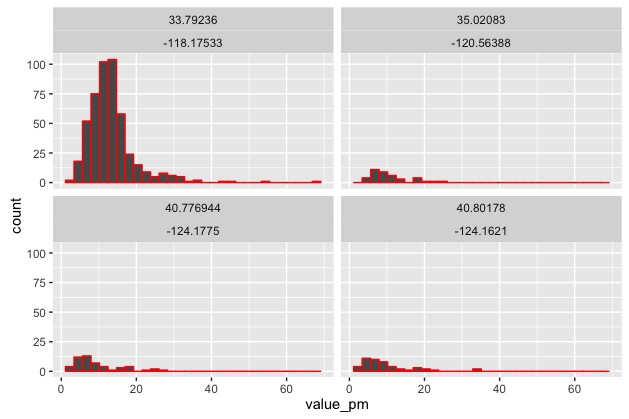
\includegraphics[width=100mm]{histpmcali.jpeg}
\caption{Histograms for $\PM$ measurements at 4 sites in California. The titles on each subpanel represent the latitudes and longitudes for the sites respectively.}
\end{figure}

The fairly skewed nature of the $\PM$ measurements, the response, and the fact that it is necessarily a positive quantity, suggest that some transformation maybe required if a Gaussian error model is to be used. Attempting to use a Gaussian model without transformation confirms this. The upper left normal QQ plot, in Figure, clearly shows a problem with the Gaussian assumption. Examining the plot on upper right of residuals versus fitted values reveals that the constant variance assumption is unreasonable. The lower left histogram of residuals confirms the pattern evident in the QQ plot: there are too many residuals in the lower tail which means that we tend to over estimate the $\PM$ levels using the model. The lower right plot emphasizes the failure of the constant variance assumption. \\ From figure 2, it is difficult to guess the appropriate transformation on the $\PM$ measurements that would alleviate this issue. We explored two options. Fitting the log transformation of the $\PM$ variable to the data tell the same story and, as before, runs into similar problems like non-constant variance and an unreasonable Gaussian assumption. The residual plots are not shown here.

\begin{figure}[h]
\centering
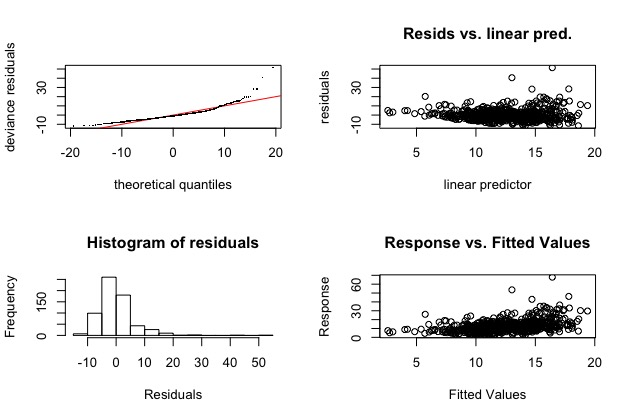
\includegraphics[width = 100mm]{gauss_diag.jpeg} 
\caption{Some basic model checking plots for a model fitted to the $\PM$ - AOD data} 
\end{figure}

\begin{figure}[h]
\centering 
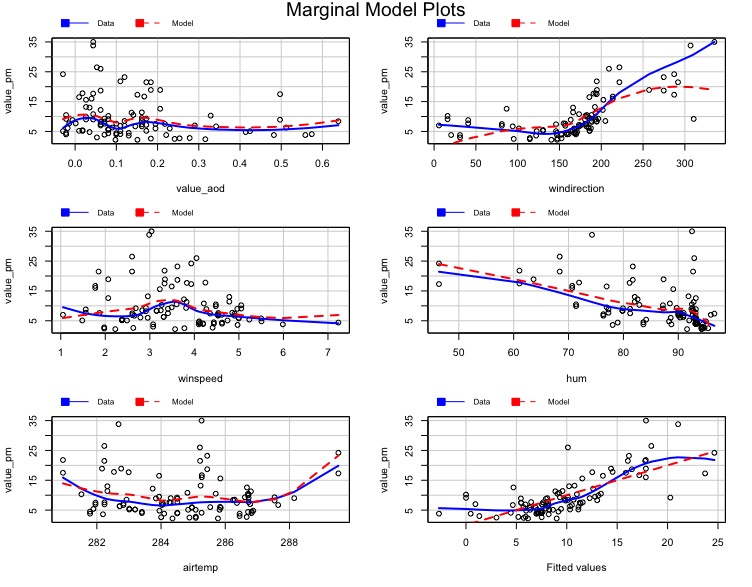
\includegraphics[width = 100mm]{mmplinreg.jpeg}
\caption{Marginal model plots for multiple linear regression}
\end{figure}

Generalized Additive Models (GAMs) employ a class of equations called "smoothers" or "scatterplot smoothers" that attempt to generalize data into smooth curves by local fitting to the subsections of the data. The basic idea behind GAMs can be described as follows. We calculate a smooth curve that goes through the data as well as possible while being parsimonious. Note that it is possible using a polynomial of high enough order to get a curve to go through every point. This makes the curve "wiggle" excessively, and not represent a parsimonious fit. The approach generally employed with GAMs is to divide the data into some number of intervals/sections, using "knots" as the end points of these intervals. Then a low order polynomial or spline function is to fit the data in an interval, with the added constraint that the second derivative of the function at the knots must be the same for both intervals sharing the knot. This eliminates sharp edges in the curve, and ensures that it is smooth and continuous at all points. As a practical matter, we can view GAMs as non-parametric curve fitters that attempt to achieve an optimal compromise between goodness-of-fit and parsimony of the final curve. One of the interesting aspects of GAMs is that they can only approximate the appropriate number of degrees of freedom, and that the number of degrees of freedom is often not an integer, but rather a real number with some fractional component. A second order polynomial (or quadratic equation) in a GLM uses two degrees of freedom (plus one for the intercept). A curve that is slightly less regular than a quadratic might require two and a half degrees of freedom (plus one for the intercept), but might fit the data better. The other aspects of GAMs that is different is that they don't handle interaction well. Rather than fit multiple variables simultaneously, the algorithm fits a smooth curve to each variable seperately and then combines the results additively, thus giving rise to the name "Generalized Additive Models. \\ \\
We model the variability in $\PM$ concentrations using generalized additive models (GAMSs) (Hastie and Tibshirani 1990). Our model can be described as follows, 
\begin{equation} 
{\mathbb{E}}(Y_{t,site} \mid AOD, U, V, H, temp, Season) = \beta_0 + \text{AOD} + f_{U}(U) + f_{V}(V) + f_{H}(H) + f_{temp}(temp) + \text{Season}  
\end{equation} 
$Y_{t, \text{site}}$ is the daily $\PM$ concentration at a given site. All the covariates vary with time and site. $\mu$ is the random model intercept, $f_{U}(U)$, $f_{V}(V)$ are one dimensional smooth surfaces describing the impact of wind speed and direction on the AOD-$\PM$ association. Season is modeled as a 4-level categorical variable because of its discrete values. \\ \\
We fit the model with the $gam()$ function in the {\textit{mgcv}} package in R (Wood 2006). The package ${mgcv}$ uses penalized regression splines for the $f_{j}$, so we can write
\begin{center} 
$f_{j}(x) = \sum \beta_{jk} {\phi_{jk}}(x) = {\bm{\beta{'}}}{\phi_j}$
\end{center} 
for the basis functions ${\phi_{jk}}$ that determine the splines. Given the basis function representation of the $f_j$, (1) is now a parametric mean function with parameters ${\bf{\beta}} = (\beta_0, {\bm{\beta_1{'}}}, \ldots, {\bm{\beta_n{'}}})^{'}$ and predictors that define the intercept and the splines that define the $s_j$.  \\
The penalized least squares objective function for estimating ${\bm{\beta}}$ is 
\begin{equation} 
{\lVert Y - X{\bm{\beta}}\rVert}^{2} + \sum_{j}\lambda_{j}{\bm{\beta_{j}{'}}}{\bm{\beta_{j}{'}}}
\end{equation}
The values of $\lambda_{j}$ are selected in an iterative algorithm to minimize a generalized cross validation criterion. This fit is done using the ${gam}$ function in the ${mgcv}$ package, 
\begin{verbatim}
Family: gaussian 
Link function: identity 

Formula:
value_pm ~ (value_aod) + s(windirection) + s(hum) + s(airtemp) + 
    season

Parametric coefficients:
            Estimate Std. Error t value Pr(>|t|)    
(Intercept)    4.085      1.065    3.84  0.00023 ***
value_aod     -2.283      2.330   -0.98  0.32993    
season         2.485      0.384    6.47  5.2e-09 ***
---
Signif. codes:  0 ‘***’ 0.001 ‘**’ 0.01 ‘*’ 0.05 ‘.’ 0.1 ‘ ’ 1

Approximate significance of smooth terms:
                 edf Ref.df     F p-value    
s(windirection) 2.66   3.28 35.38 < 2e-16 ***
s(hum)          2.46   3.00  1.37 0.24676    
s(airtemp)      3.07   3.81  5.73 0.00051 ***
---
Signif. codes:  0 ‘***’ 0.001 ‘**’ 0.01 ‘*’ 0.05 ‘.’ 0.1 ‘ ’ 1

R-sq.(adj) =  0.786   Deviance explained = 80.8%
GCV = 11.065  Scale est. = 9.8282    n = 100
\end{verbatim} 
The only visible parameter in this model is the intercept, estimated to be 4.085. The ${\bm{\beta_{j}}}$ are hidden inside the smoothers and are largely uninterpretable. For each of its predictors, a smoother was fit by the $f$ functions. The default in the function $f$ that does the smoothing uses {\textit{thin plate regression splines}} that don't depend as much on the number of knots selected and also they generalize to smooths of more than one variable at a time. In the output, the "edf" is the equivalent degrees of freedom for each of the smooths. If we are using $k$ basis functions for a smooth, then we would have $k$ degrees of freedom (df) for the smooth. Penalization will generally reduce edf to a number smaller than $k$. The adjusted $R^{2}$ is the square of the correlation between the observed and fitted values, with an adjustment for degree of freedom, while the deviance explained appears to be the usual $R^2$. 



\begin{figure}[h]

\centering
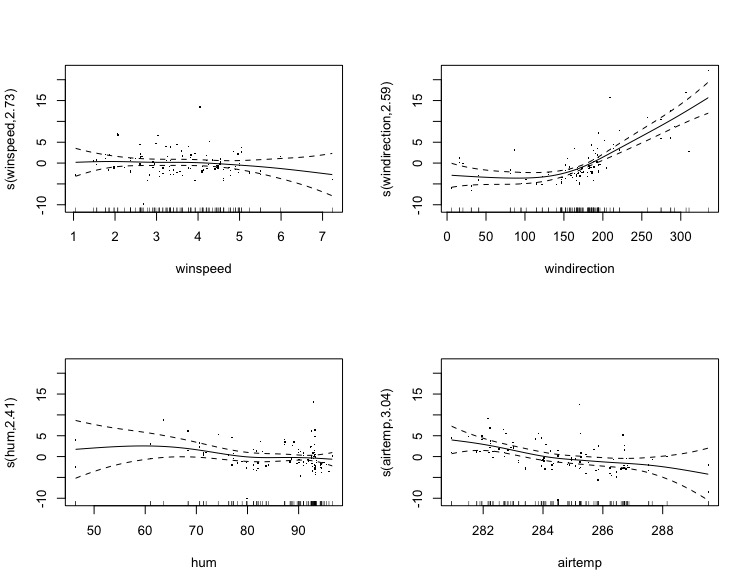
\includegraphics[width = 90mm]{pred.jpeg} 
\caption{The estimates of the smooth functions shown without partial residuals. The dotted lines aound the solid lines show the Bayesian credible intervals.} 
\end{figure} 
In Figure 4, the solid line is the predicted value of the dependent variable as a function x axis. We plot two times the standard errors of the estimates (in dashed lines). The small lines along the x axis are the "rugs" showing the location of the sample plots. The result for all the predictors look relatively flat because the standard errors are not too large. \\ 
We also perform the likelihood ratio tests to compare different models and conclude that the model displayed on the previous page does the best job. 











%%%%%%%%%%%%%%%%%%%%%%%%%%%%%%%


%\begin{verbatim} 
%Family: Gamma 
%Link function: log 
%
%Formula:
%value_pm ~ (value_aod) + s(winspeed, windirection) + s(hum) + 
%    s(airtemp) + season
%
%Parametric coefficients:
%            Estimate Std. Error t value Pr(>|t|)    
%(Intercept)   2.1283     0.0538   39.59  < 2e-16 ***
%value_aod     0.3666     0.1579    2.32    0.021 *  
%season        0.1386     0.0196    7.06  4.8e-12 ***
%---
%Signif. codes:  0 ‘***’ 0.001 ‘**’ 0.01 ‘*’ 0.05 ‘.’ 0.1 ‘ ’ 1
%
%Approximate significance of smooth terms:
%                           edf Ref.df    F p-value    
%s(winspeed,windirection) 21.46  25.55 8.11  <2e-16 ***
%s(hum)                    7.50   8.41 1.95   0.044 *  
%s(airtemp)                4.24   5.26 2.56   0.024 *  
%---
%Signif. codes:  0 ‘***’ 0.001 ‘**’ 0.01 ‘*’ 0.05 ‘.’ 0.1 ‘ ’ 1
%
%R-sq.(adj) =  0.266   Deviance explained = 36.2%
%GCV = 0.17517  Scale est. = 0.17318   n = 630
%\end{verbatim} 
%
%$R^2 = .266$ is low since this analysis has been conducted for 4 sites in California. The cross-validation error is not too bad either. These values significantly improve considerably when we consider one site at a time. Doing an analysis of variance on the model (see below) shows that the two variables that significantly affect the $\PM$ levels are temperature and wind velocity. \newpage


%\begin{figure}[h]
%\centering
%\begin{subfigure}{.5\textwidth}
%\centering
%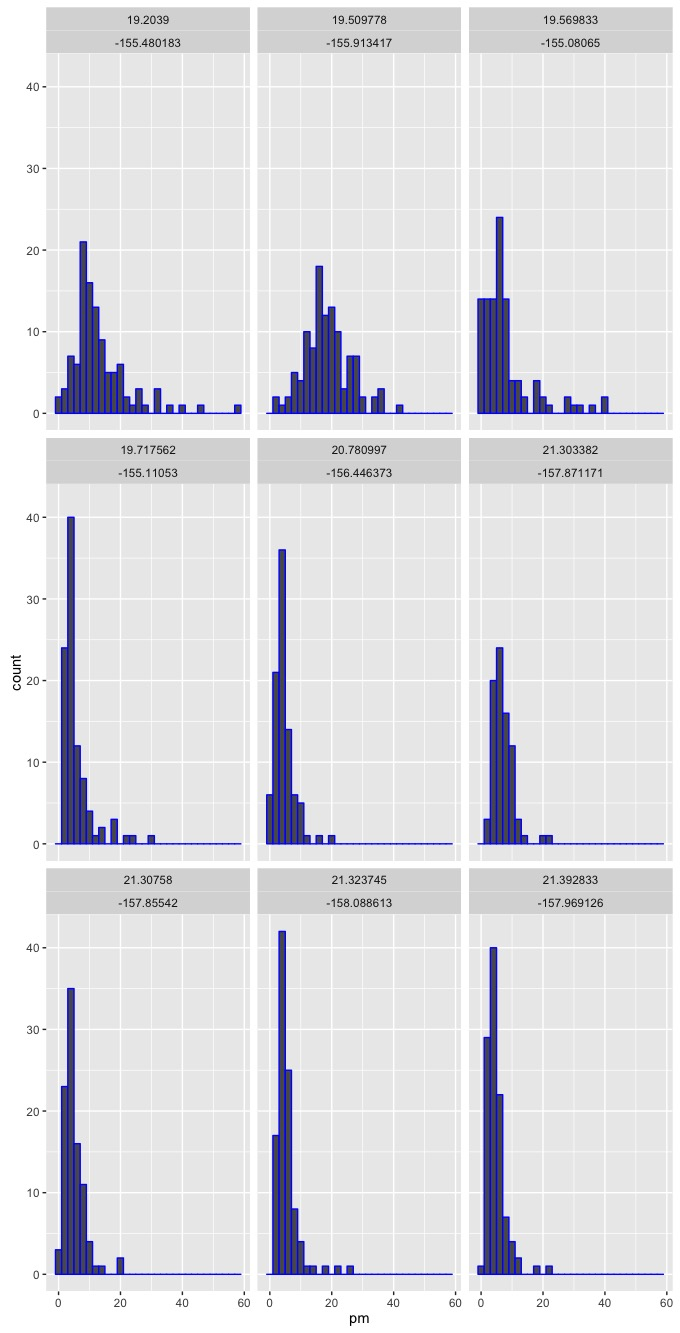
\includegraphics[width = .4\linewidth]{hist_hawa.jpeg}
%\caption{$\PM$ concentrations from 9 ground monitoring sites}
%\label{histpm}
%\end{subfigure}	
%\begin{subfigure}{.4\textwidth}
%\centering
%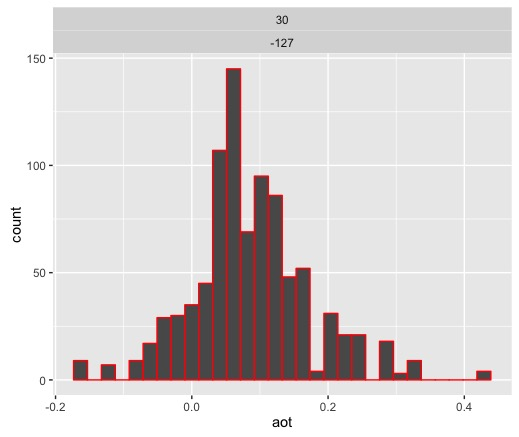
\includegraphics[width = .5\textwidth]{histaod_hawa.jpeg}
%\caption{AOD measurements from the satellite} 
%\end{subfigure}
%\caption{Histograms of the measurements at 9 sites in Hawaii} 
%\end{figure} 






\end{itemize}





\end{document}